\documentclass[10pt,a4paper]{article}
\usepackage[lmargin=3.0cm,rmargin=3.0cm,tmargin=3.0cm,bmargin=3.0cm,head=2cm,headsep=0.5cm]{geometry}
\setlength\parindent{0pt}
\usepackage[utf8]{inputenc}
\usepackage{amssymb}
\usepackage{color}
\usepackage[ngerman]{babel}
\usepackage{here} 
\usepackage{graphicx}
\graphicspath{{./images/} }
\usepackage[hang]{footmisc}
\linespread{1.5}
\usepackage{listings} \lstset{numbers=left, numberstyle=\tiny, numbersep=5pt} 
\definecolor{code}{rgb}{0.94, 0.97, 1.0}
\definecolor{red}{rgb}{1.0, 0.03, 0.0}
\definecolor{green}{rgb}{0.0, 0.65, 0.31}
\usepackage{hyperref}
\lstset{
	  basicstyle=\ttfamily,
	  breaklines=true,
	  numberstyle=\footnotesize,
      numbersep=5pt,   
	  literate={Ö}{{\"O}}1 {Ä}{{\"A}}1 {Ü}{{\"U}}1 {ß}{{\ss}}2 {ü}{{\"u}}1 {ä}{{\"a}}1 {ö}{{\"o}}1 {µ}{\textmu}1,
      columns=fullflexible,
      language=Java,
      showstringspaces=false,
      commentstyle={\color{green}},
      keywordstyle=\color{black},
      stringstyle=\color{red},
      extendedchars=\true,
      tabsize=4,
      breaklines=true,
      breakatwhitespace=true,
      backgroundcolor=\color{code}} 

\title{IT-Projekt}

\begin{document}

\begin{titlepage}
\vspace*{1cm}
\begin{center}
\Huge
Technische Hochschule Nürnberg\\
\vspace*{2cm}
\large
IT-Projekt\\ Verteiltes Erdbebenwarnsystem\\
Bearbeitungszeitraum: SS13 - WS13/14\\
\vspace*{2cm}
\Huge
IT Projekt\\
\vspace{1cm}
\large
\vspace{2cm}

 \begin{tabular}{p{6 cm}p{6 cm}}
    	vorgelegt von & {Christopher Althaus} \\
		& {Baris Akdag} \\
		& {Niklas Schäfer} \\
		& {Benjamin Brandt} \\
		& {Jürgen Hetzel} \\ & \\
    	Betreuer & {Prof. Dr. Michael Zapf}\\ & \\
    	Abgabe:& 14. Februar 2014
 \end{tabular}\\
    


\end{center}
\end{titlepage}


\newpage

\clearpage\thispagestyle{empty}
\begin{center}\textbf{\large Erklärung}\end{center}

\noindent
Hiermit versichern wir, dass wir die Arbeit selbständig verfasst, nicht anderweitig für Prüfungszwecke vorgelegt, alle benutzten Quellen und Hilfsmittel angegeben 
sowie wörtliche und sinngemäße Zitate als solche gekennzeichnet zu haben. \\
\\ \\ \\ \\
\begin{tabular}{l}
 \\ \\ \\
\line(1,0){165}\\
Christopher Althaus\\
 \\ \\ \\
\line(1,0){165}\\
Baris Akdag\\
 \\ \\ \\
\line(1,0){165}\\
Niklas Schäfer\\
 \\ \\ \\
\line(1,0){165}\\
Benjamin Brandt\\
 \\ \\ \\
\line(1,0){165}\\
Jürgen Hetzel \qquad \qquad \qquad \qquad \qquad  \qquad  \qquad  \qquad \qquad  \qquad   
Nürnberg, den \today
\end{tabular}
\newpage
\begin{center}\textbf{\large Abstract}\end{center}
Portable Geräte wie aktuelle Smartphones und Tablet-Computer besitzen in der Regel eine Vielzahl von Sensoren, darunter auch solche, die Beschleunigungen feststellen können. Diese können insbesondere genutzt werden, um Erschütterungen des Geräts festzustellen. Die unten gezeigte Grafik ist die Ausgabe einer Android-Anwendung (App), welche diese Sensoren ausliest.\\
Offensichtlich werden diese Sensoren ständig ausgelöst, wenn der Benutzer das Gerät mit sich führt, während er sich fortbewegt. Dabei sind die Werte der Sensoren unmittelbar von der individuellen Bewegung abhängig und daher stets zwischen zwei Geräten verschieden.\\
Interessant wäre es, wenn es möglich wäre, Korrelationen zwischen den Sensorwerten auf verschiedenen Geräten zu finden. Dies würde darauf hindeuten, dass beide Geräte, zumal wenn sie an verschiedenen Orten aufbewahrt werden, dasselbe Ereignis wahrgenommen haben, etwa eine Erschütterung im Boden. \\
Dies könnte dazu genutzt werden, um ein automatisches Erdbebenmeldesystem zu realisieren. Wenn eine gewisse Menge von Geräten zur gleichen Zeit ein ähnliches Erschütterungsmuster detektieren, ist davon auszugehen, dass sich ein Erdbeben ereignet. Dies wird natürlich von den Anwendern selbst auch bemerkt werden, jedoch könnten die Geräte einerseits einen Alarm auslösen, der auch solche Menschen warnt, die aus diversen Gründen das Ereignis nicht wahrnehmen (schlafen oder im Auto sitzen), andererseits könnten Sicherheitsmaßnahmen in Gang gesetzt werden (automatisches Abstellen der Gasversorgung, Abstellen des Stroms an gefährlichen Orten usw.).
\newpage
\tableofcontents
\newpage
\section{Teamorganisation}
Die Projektgruppe besteht aus Niklas Schäfer, Baris Akdag, Christopher Althaus, Benjamin Brandt sowie Jürgen Hetzel. Innerhalb der Gruppe sind zu Beginn die verschiedenen Aufgabengebiete nach Interessen und Fähigkeiten des einzelnen verteilt worden.\\
Baris Akdag verfügte im Vorfeld über Fachkenntnisse in den Bereichen WebServices und Datenbanken. Er übernahm die Entwicklung des gesamten WebServices inklusive Datenbank und Bereitstellung.\\
Durch die Erfahrung von Christopher Althaus im Bereich Android Programmierung bot er sich neben Niklas Schäfer an, die Android Applikation zu entwicklen.\\
Dabei übernahm Niklas Schäfer als Hauptaufgaben die Lokalisierung der Geräte inklusive der Sicherstellung aktivierter Standortbestimmung auf den Smartphones, sowie die Einbindung und Weiterentwicklung der Google Maps Karte. Weiterhin implementierte er die Einstellungen (Settings View und deren Funktion) und arbeitete am User Interface der App.\\ 
Christopher Althaus widmete sich neben der groben Strukturierung der App, hauptsächlich um die Aufgabengebiete rund um den Beschleunigungssensor und um die Benutzerbenachrichtigung im Falle eines Erdbebens. Diese Aufgaben umfassten zum Einen die Erdbebenerkennung innerhalb der Applikation und zum anderen die Einbindung eines Diagramms zur Visualisierung der Beschleunigungsdaten.\\
Jürgen Hetzel und Benjamin Brand übernahmen während des Projektablaufs einen Großteil der Literaturrecherche. Ebenso befasste sich Jürgen Hetzel mit einer Teilaufgabe für die App Einstellungen, erstellte das Tablet-Layout und kümmerte sich zum Ende des Projekts um das Refactoring der Android Applikation.
Da Benjamin Brand über eine große Auswahl von Geräten verfügte, übernahm er zusätzlich das Testen der Anwendung.\\
Über den gesamten Zeitraum der Bearbeitung ist eine enge Zusammenarbeit und gute Kommunikation Grundlage für ein erfolgreiches Umsetzen des Projekts gewesen.
\newpage
\section{Motivation}
\section{System Struktur}
Die Erdbebenerkennung soll über ein verteiltes System erfolgen. Prinzipiell handelt es sich hierbei um ein Client-Server-System, wobei die Android Smartphones die Clients darstellen. Den Teil des Servers soll ein WebService übernehmen. Die die Strukturierung und Kommunikationsbeziehung dieser beiden Komponenten ist in Abbildung \ref{fig:SystemStrukutr} dargestellt.
\begin{figure}[H]
\centering
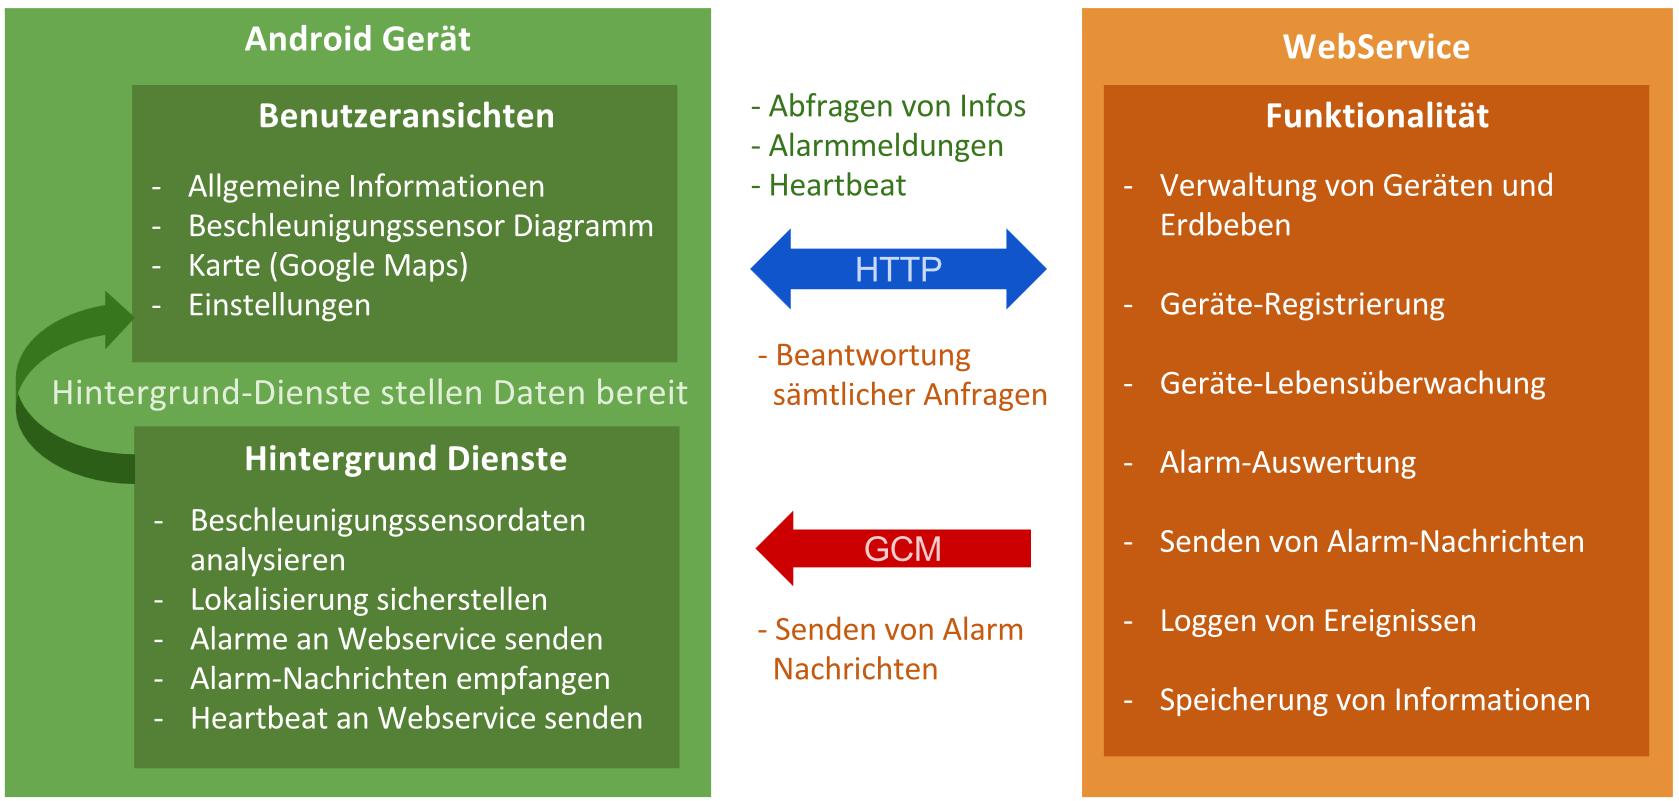
\includegraphics[width=\textwidth]{/Systemstruktur.png}
\caption{Struktur des Projektes}
\label{fig:SystemStrukutr}
\end{figure}
Das rechts dargestellte Android Gerät kann grundlegend in die Benutzeransichten und Hintergrund-Dienste unterteilt werden. 

\section{Erdbebenerkennung unter Android}
\section{Fazit}
Zusammengenommen ist in dem Projekt das gewünschte Ergebnis erreicht worden. Alle wesentlichen Anforderungen konnten umgesetzt werden. Das Projekt erforderte eine tiefgehende Auseinandersetzung in die Android und WebService Programmierung unter Java. Ebenso sind die Kompetenzen im Bereich der Teamarbeit bei allen Beteiligen erweitert worden.\\
Abschließend kann festgestellt werden, dass diese Lösung zur Erdbebenerkennung durchaus sinnvoll eingesetzt werden kann und eines Tages dazu dienen könnte, Sach- und Personenschäden bei einem Erdbeben zu minimieren.
\newpage
\end{document}

